
\begin{frame}
  \frametitle{Pre-detonation Materials of Interest}
  \begin{itemize}
    \item UOC
    \item UOX powder
    \item SNF
    \item Reprocessed SNF
    \item Separated Pu
    \item Anything radioactive from the fuel cycle
  \end{itemize}
\end{frame}

\begin{frame}
  \frametitle{Statistical Methods Employed}
  \begin{minipage}[t]{0.45\textwidth}
    \begin{figure}
      \raggedleft
      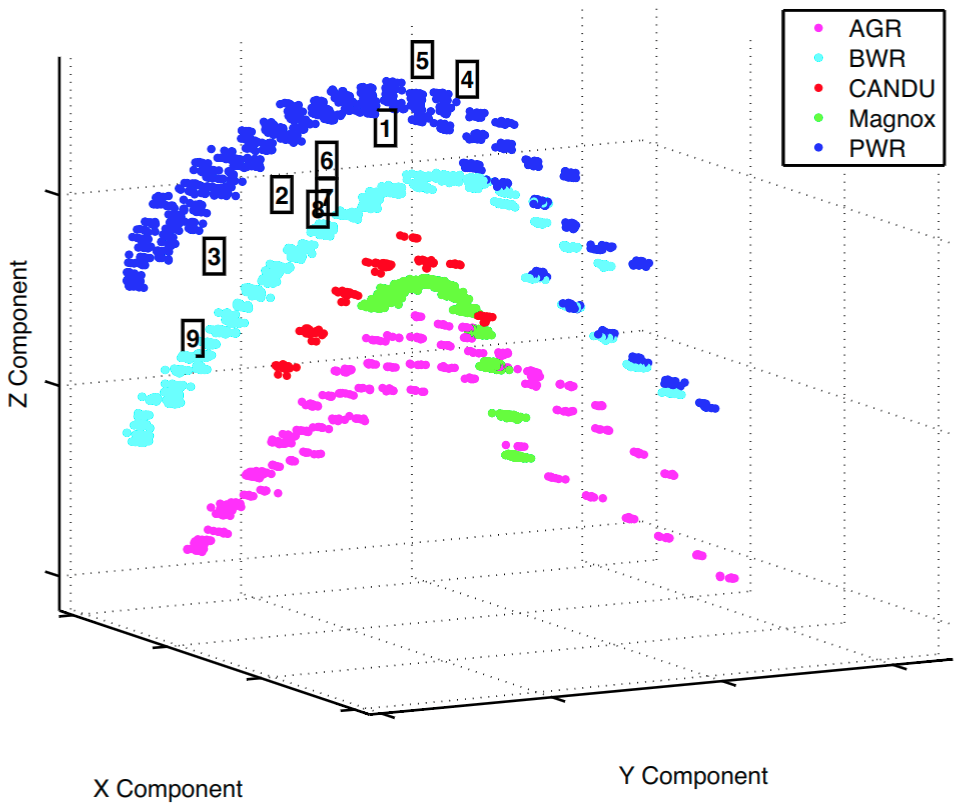
\includegraphics[width=1\linewidth]{./figures/sfcompo.png}
      \caption{Unsupervised clustering for visualization separating reactor types \cite{jones_viz_2014}}
    \end{figure}
  \end{minipage}\hfill
  \begin{minipage}[t]{0.45\textwidth}
    \begin{figure}
      \raggedright
      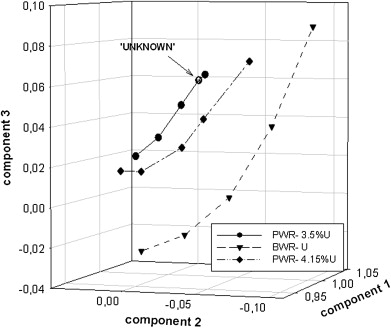
\includegraphics[width=1\linewidth]{./figures/nicolaou.jpg}
      \caption{Factor analysis employed to determine provenance of unknown plutonium \cite{nicolaou_pu}}
      %\caption{Factor Analysis \cite{nicolaou_2006, nicolaou_pu, nicolaou_2014, nicolaou_2009, nicolaou_2015}}
    \end{figure}
  \end{minipage}
\end{frame}

\begin{frame}
  \frametitle{Statistical Methods Employed}
  \begin{figure}
    \centering
    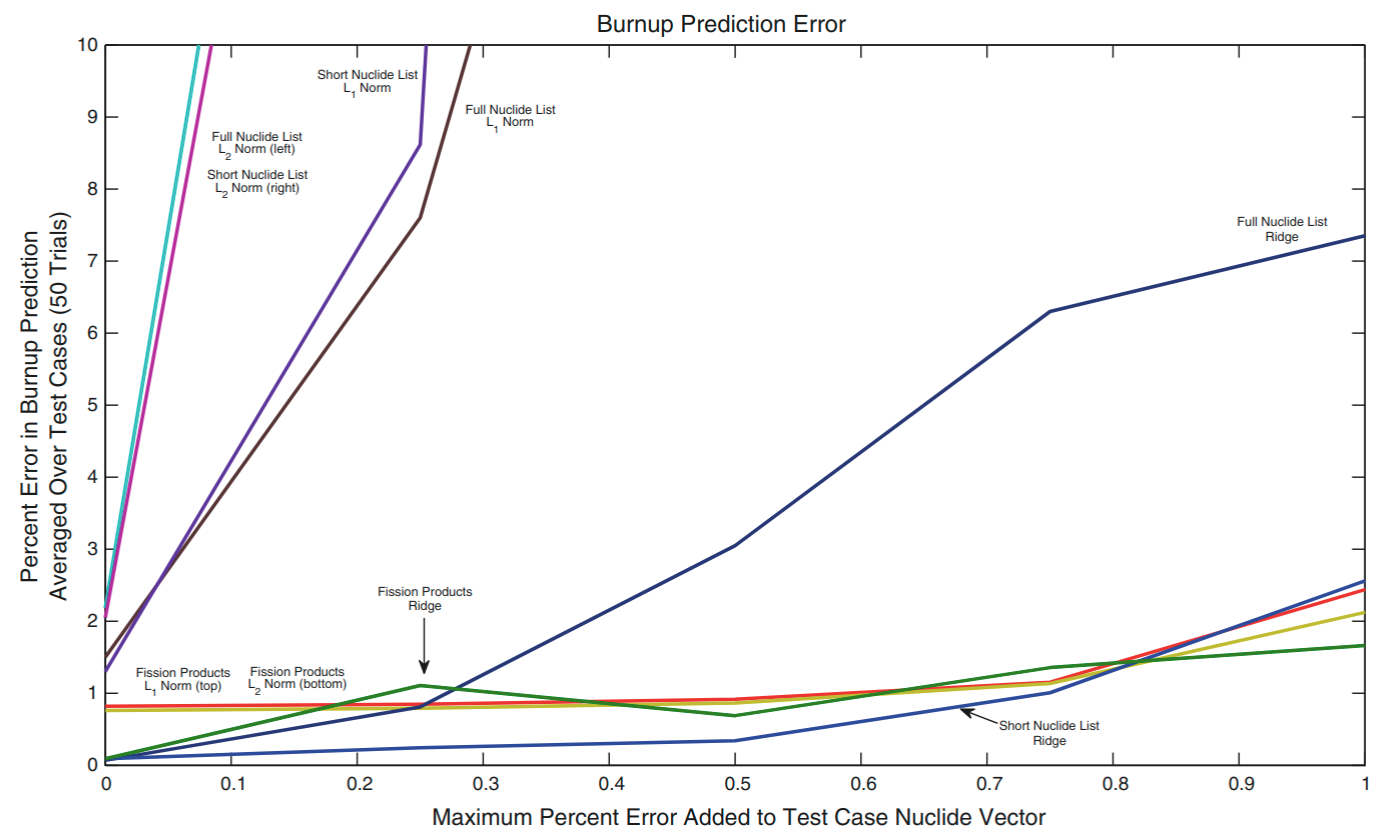
\includegraphics[width=0.85\textwidth]{./figures/randomerror.png}
    \caption{Burnup prediction error with respect to random nuclide error, using nearest neighbor \& ridge regression methods \cite{dayman_feasibility_2013}}
  \end{figure}
\end{frame}
